
我們知道為了有效地使用處理器,必須有足夠的代碼來並行執行多條指令。沒有足夠的指令來保持CPU繁忙的主要原因可能是數據依賴,由於輸入沒有準備好,無法運行指令。通過流水線可以來解決這個問題,但必須事先知道哪些指令將執行。處理這個問題的方法是,根據計算這個條件的歷史走向,對是否採用條件分支進行有根據的猜測。猜測越可靠,性能越好。猜測不可靠時,性能會受到嚴重影響。

所有這些性能問題的根源是條件分支,下一條要執行的指令直到運行時才知道。這個問題的根本解決方案是重寫我們的代碼,不使用分支,或者更少的分支。這就是\textbf{無分支計算}。

\subsubsubsection{3.8.1\hspace{0.2cm}循環展開}

事實上,這個想法並不新穎。瞭解了分支影響性能的機制,因此使用循環展開技術來減少分支數量。回到我們最初的代碼示例:

\begin{lstlisting}[style=styleCXX]
for (size_t i = 0; i < N; ++i) {
	a1 += p1[i] + p2[i];
}
\end{lstlisting}

雖然循環體是完全流水的,但是這段代碼中有一個隱藏的分支:循環檢查的結束,這個檢查在每個循環迭代中執行一次。若事先知道,迭代次數N是偶數,就不需要在奇數次迭代後執行檢查,可以顯式地省略這個檢查:

\begin{lstlisting}[style=styleCXX]
for (size_t i = 0; i < N; i += 2) {
	a1 += p1[i] + p2[i]
		+ p1[i+1] + p2[i+1];
}
\end{lstlisting}

展開循環,將兩個迭代轉換為一個更大的迭代。這個例子和其他類似的例子一樣,手動展開不太可能提高性能。首先,如果N很大,循環分支的結束部分可以完美地預測出來。其次,編譯器可能會將展開作為一種優化,矢量化編譯器將使用SSE或AVX指令來實現這個循環。實際上,這裡對循環體進行展開的原因是,向量指令一次可以處理多個數組元素,不過這些結論都需要通過基準測試或分析來確認。如果發現手動循環展開對性能沒有影響,不要感到驚訝(我們對於分支的理解沒有問題),這意味著原始代碼已經進行了循環展開,這個優化操作已經由編譯器完成了。

\subsubsubsection{3.8.2\hspace{0.2cm}無分支選擇}

循環展開是一個非常特殊的優化,編譯器會來做這件事。將展開的想法轉化為無分支計算是最近的進展,可以帶來驚人的性能收益。我們將從一個非常簡單的例子開始:

\begin{lstlisting}[style=styleCXX]
unsigned long* p1 = ...; // Data
bool* b1 = ...; // Unpredictable condition
unsigned long a1 = 0, a2 = 0;
for (size_t i = 0; i < N; ++i) {
	if (b1[i]) {
		a1 += p1[i];
	} else {
		a2 += p1[i];
	}
}
\end{lstlisting}

假設條件變量\texttt{b1[i]}不能由處理器預測,這段代碼的運行速度比良好的分支預測循環慢幾倍。這裡可以做得更好,就是可以完全消除這個分支,並通過指向兩個目標變量的指針數組,通過索引來進行替換:

\begin{lstlisting}[style=styleCXX]
unsigned long* p1 = ...; // Data
bool* b1 = ...; // Unpredictable condition
unsigned long a1 = 0, a2 = 0;
unsigned long* a[2] = { &a2, &a1 };
for (size_t i = 0; i < N; ++i) {
	a[b1[i]] += p1[i];
}
\end{lstlisting}

轉換中,利用了布爾變量只能有兩個值(0(\texttt{false})或1(\texttt{true})),將其轉換為整數(如果用其他類型代替\texttt{bool},必須確保所有的真值都由1表示,因為任何非零值都認為是真值,但只有1的值在我們的無分支代碼中有效)。

這個轉換通過對兩個內存位置中的一個進行條件訪問,替換掉指令中的條件跳轉。由於這種條件內存訪問可以流水化,無分支的版本具有顯著的性能改善:

%\hspace*{\fill} \\ %插入空行
\begin{center}
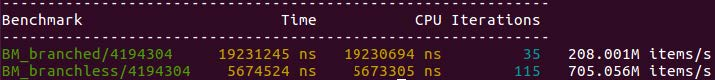
\includegraphics[width=0.9\textwidth]{content/1/chapter3/images/30.jpg}\\
圖 3.30
\end{center}

這個例子中,無分支的代碼版本要快3.5倍。有些編譯器在可能的情況下使用查找數組,而不使用條件分支來實現\texttt{?:}操作符。使用這樣的編譯器,可以通過如下循環體獲得相同性能:

\begin{lstlisting}[style=styleCXX]
for (size_t i = 0; i < N; ++i) {
	(b1[i] ? a1 : a2) += p1[i];
}
\end{lstlisting}

通常,確定這種優化是否有效或效果如何的唯一方法是測試。

前面的例子涵蓋了無分支計算的所有基本元素:不是有條件地執行這個或那個代碼,而是轉換它們,使代碼在所有情況下都相同,條件邏輯由索引操作實現。我們將通過更多的例子來強調一些事項和限制。

\subsubsubsection{3.8.3\hspace{0.2cm}無分支的例子}

大多數時候,依賴於條件的代碼並不簡單。通常,必須根據一些中間值來進行不同的計算:

\begin{lstlisting}[style=styleCXX]
unsigned long *p1 = ..., *p2 = ...; // Data
bool* b1 = ...; // Unpredictable condition
unsigned long a1 = 0, a2 = 0;
for (size_t i = 0; i < N; ++i) {
	if (b1[i]) {
		a1 += p1[i] - p2[i];
	} else {
		a2 += p1[i] * p2[i];
	}
}
\end{lstlisting}

條件影響計算的表達式和結果存儲的位置。兩個分支唯一的共同之處就是輸入,通常情況下,即使是輸入也不一定是這樣。

為了在沒有分支的情況下計算出相同的結果,必須從條件變量索引的內存位置獲取正確表達式的結果。因為我們決定不根據條件更改執行的代碼,所以兩個表達式都將執行。這樣,向無分支的轉換就很簡單了:

\begin{lstlisting}[style=styleCXX]
unsigned long a1 = 0, a2 = 0;
unsigned long* a[2] = { &a2, &a1 };
for (size_t i = 0; i < N; ++i) {
	unsigned long s[2] = { p1[i] * p2[i], p1[i] - p2[i] };
	a[b1[i]] += s[b1[i]];
}
\end{lstlisting}

兩個表達式都執行了,結果存儲在一個數組中。該數組用於索引計算的目標,即遞增的變量。這增加了循環體的計算量,由於是連續的代碼,沒有了跳轉,所以只要CPU有資源做更多的操作,這裡的性能就會有提升。基準測試證實了這種無分支轉換確實有效:

%\hspace*{\fill} \\ %插入空行
\begin{center}
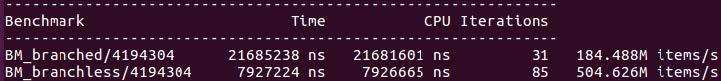
\includegraphics[width=0.9\textwidth]{content/1/chapter3/images/31.jpg}\\
圖 3.31
\end{center}

額外計算的數量有限,而且仍然優於條件代碼。這裡甚至沒有一個通用型經驗法則可以用來進行猜測(無論如何,都不應該猜測性能)。必須測量這種優化的有效性,它高度依賴於代碼和數據。若分支預測器非常有效(可預測的條件,而不是隨機條件),那麼條件代碼將優於無分支的版本:

%\hspace*{\fill} \\ %插入空行
\begin{center}
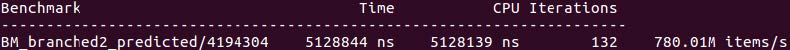
\includegraphics[width=0.9\textwidth]{content/1/chapter3/images/32.jpg}\\
圖 3.32
\end{center}

可以從圖3.31和圖3.32中得到的結論是,流水線刷新(錯誤預測的分支)的成本有多高,以及CPU在指令級並行性的同時可以做多少計算。無分支計算依賴的是隱藏的和未使用的計算資源,可能還沒有耗盡這個資源(在我們的示例中)。我們可以展示代碼的無分支轉換的另一個版本,不使用數組來選擇正確的結果變量,如果不想改變結果,將兩者加零:

\begin{lstlisting}[style=styleCXX]
unsigned long a1 = 0, a2 = 0;
for (size_t i = 0; i < N; ++i) {
	unsigned long s1[2] = { 0, p1[i] - p2[i] };
	unsigned long s2[2] = { p1[i] * p2[i], 0 };
	a1 += s1[b1[i]];
	a2 += s2[b1[i]];
}
\end{lstlisting}

現在有兩個中間值的數組,而不是目標數組。這個版本會無條件地進行更多的計算,並且具有與之前無分支代碼相同的性能:

%\hspace*{\fill} \\ %插入空行
\begin{center}
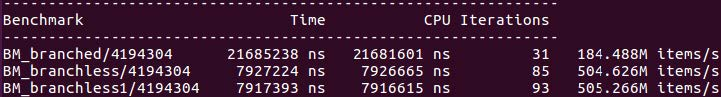
\includegraphics[width=0.9\textwidth]{content/1/chapter3/images/33.jpg}\\
圖3.33 - 圖3.31的結果,為另一個無分支實現添加了“BM\_branchless1”
\end{center}

理解無分支變換的侷限性是很重要的,不要忘乎所以。我們已經看到了一個限制:無分支代碼通常要執行更多指令。因此,如果分支預測器工作良好,那麼少量的流水刷新可能不足以證明優化的合理性。

無分支轉換不能按預期執行的第二個原因與編譯器有關:在某些情況下,編譯器可以進行等效或更好的優化。例如\textbf{鉗位環(clamp loop)}:

\begin{lstlisting}[style=styleCXX]
unsigned char *c = ...; // Random values from 0 to 255
for (size_t i = 0; i < N; ++i) {
	c[i] = (c[i] < 128) ? c[i] : 128;
}
\end{lstlisting}

該循環將\texttt{unsigned char}數組\texttt{c}的值限制為128。初始值是隨機的,循環體中的條件在任何程度上都不能預測,可以預期一個非常高的分支錯誤預測率。另一種無分支的實現使用具有256個元素的\textbf{查找表(LUT)},每個元素對應一個\texttt{unsigned char}值。索引\texttt{i}從0到127的表項\texttt{LUT[i]}包含索引值本身,更高索引值的在\texttt{LUT[i]}中為128:

\begin{lstlisting}[style=styleCXX]
unsigned char *c = ...; // Random values from 0 to 255
unsigned char LUT[256] = { 0, 1, …, 127, 128, 128, … 128 };
for (size_t i = 0; i < N; ++i) {
	c[i] = LUT[c[i]];
}
\end{lstlisting}

大多數現代編譯器,這根本不是優化問題:編譯器可以更好地處理原始代碼,很可能使用SSE或AVX向量指令一次複製和多個鉗位字符,從而不需要任何分支。我們對原始代碼進行了剖析(而不是假設分支必須錯誤預測),發現該程序不會受到分支預測的影響。

還有一種情況是,無分支轉換可能不成功,即循環體的開銷明顯高於分支(即使是錯誤的預測分支)。這種情況值得注意,因為它經常會在循環中使用:

\begin{lstlisting}[style=styleCXX]
unsigned long f1(unsigned long x, unsigned long y);
unsigned long f2(unsigned long x, unsigned long y);
unsigned long *p1 = ..., *p2 = ...; // Data
bool* b1 = ...; // Unpredictable condition
unsigned long a = 0;
for (size_t i = 0; i < N; ++i) {
	if (b1[i]) {
		a += f1(p1[i], p2[i]);
	} else {
		a += f2(p1[i], p2[i]);
	}
}
\end{lstlisting}

根據條件\texttt{b1},我們調用兩個函數中的一個,\texttt{f1()}或\texttt{f2()}。如果使用函數指針數組,可以消除\texttt{if-else}語句,可以使代碼無分支:

\begin{lstlisting}[style=styleCXX]
decltype(f1)* f[] = { f1, f2 };
for (size_t i = 0; i < N; ++i) {
	a += f[b1[i]](p1[i], p2[i]);
}
\end{lstlisting}

這是值得做的優化嗎?通常情況下,並不是。首先,如果可以內聯\texttt{f1()}或\texttt{f2()},那麼函數指針調用將阻止這種情況。內聯通常是一個主要的優化,放棄內聯來擺脫分支是不合理的。函數沒有內聯,函數調用本身就破壞了流水(這是內聯是有效的優化的一個原因)。與函數調用的成本相比,即使是一個錯誤的分支預測通常也沒有那麼多性能開銷。

儘管如此,有時函數查找表也是值得優化的:它從不只提供兩個選項,但是如果必須基於一個條件從多個函數中進行選擇,那麼函數指針表比鏈式\texttt{if-else}語句更有效。值得注意的是,這個示例與所有現代編譯器用於實現虛函數調用的實現非常相似,調用也使用函數指針數組(而不是比較鏈)。如果需要優化基於運行時條件,調用多個函數中的一個,則應該考慮是否應該使用多態對象進行重新設計。

還應該記住無分支轉換對代碼可讀性的影響:函數指針的查找表不容易讀懂,調試起來可能比開關或if-else語句困難得多。由於影響最終結果的因素很多(編譯器優化、硬件資源可用性、程序操作數據的屬性),任何優化都必須通過基準測試和概要數據文件之類的測量進行驗證,並權衡其源碼對於開發者的開發時間、可讀性和複雜性。






